%----------------------------------------------------------------------------------------
%	Cover, copyright and ToC
%----------------------------------------------------------------------------------------

\begingroup
\thispagestyle{empty}

\AddToShipoutPicture*{\put(0,0)\centering{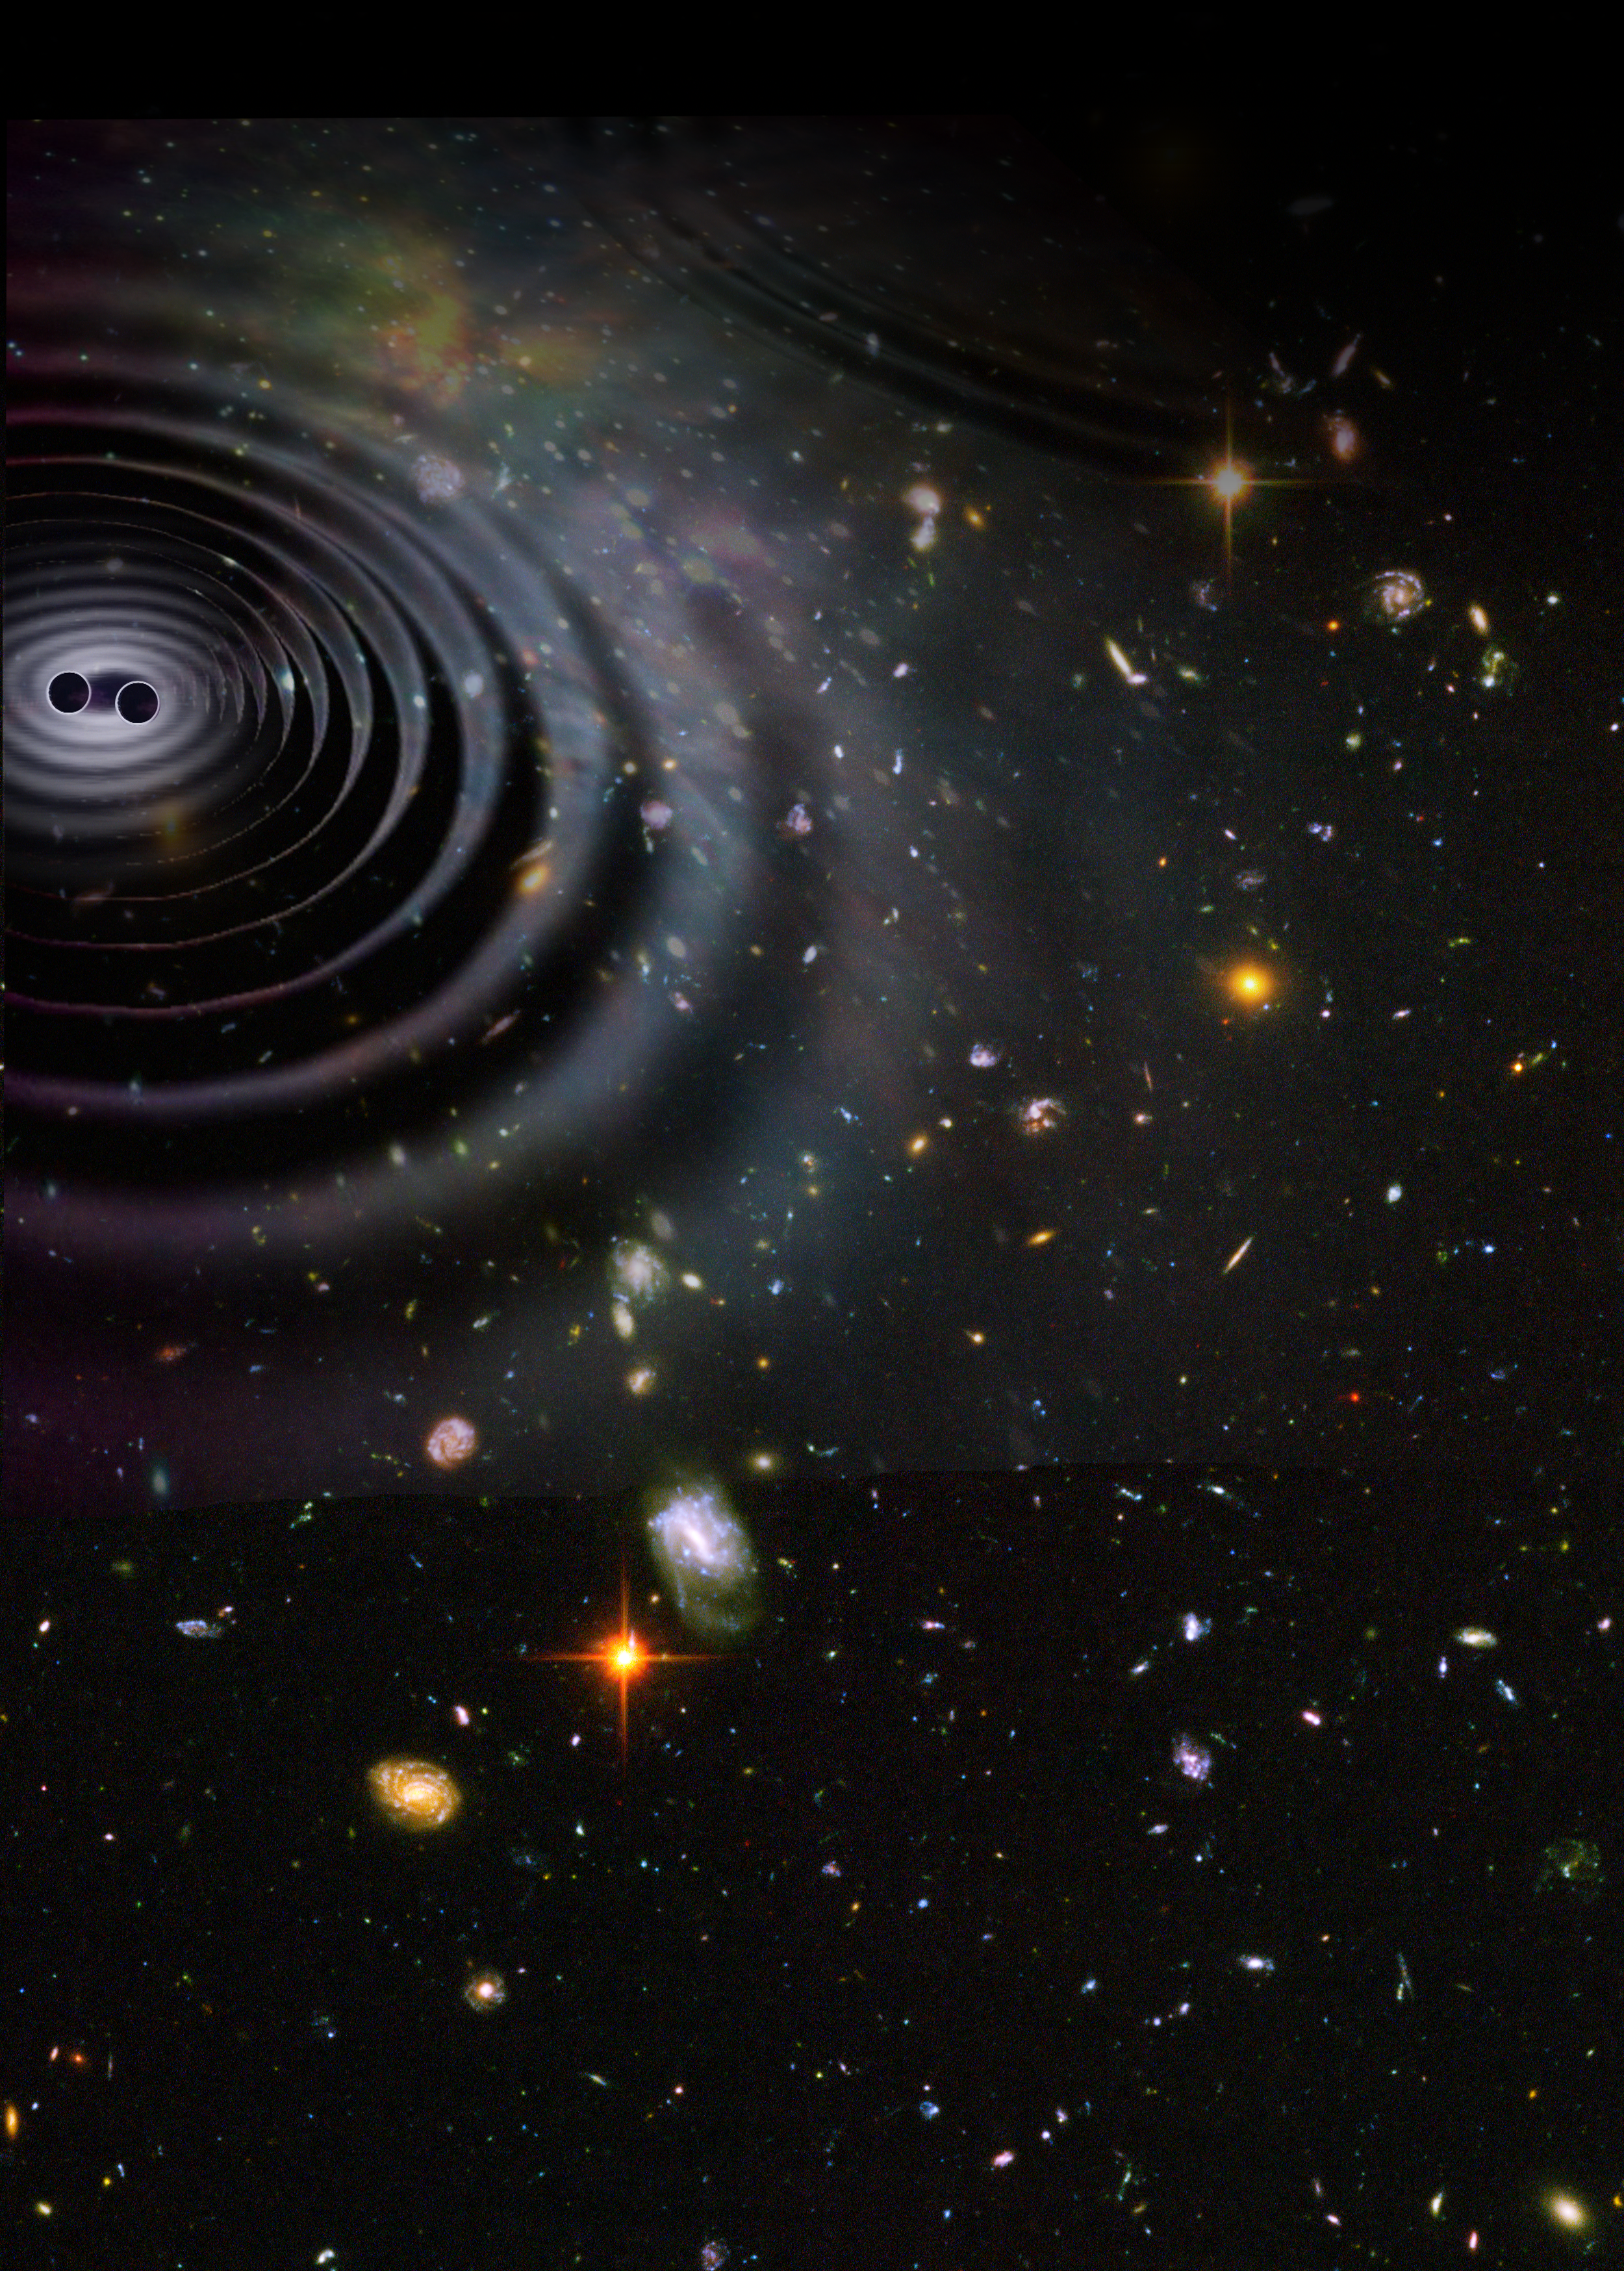
\includegraphics[width=1.45\textwidth]{Figures/Cover.png}}} % Image from ET Design study Mix of input from NIKHEF, Hubble ultra deep field (NASA), Waves: Bernard Schutz, black holes + waves Harald Lueck, composed and edited Harald Lueck
\centering
\par\normalfont\fontsize{1}{1}\sffamily\selectfont
\textcolor{black}{\textbf{.}}\\ %trick for putting the title a little lower on the page
\vspace{2.5cm}
\par\normalfont\fontsize{60}{60}\sffamily\selectfont
\textcolor{yellow}{\textbf{3G R\&D}}\\
\vskip6cm
\par\normalfont\fontsize{25}{25}\sffamily\selectfont
\textsc{\textcolor{yellow}{{R\&D for the next generation of ground-based gravitational-wave detectors}}}\par % Book title
\vskip7.5cm
\textcolor{yellow}{\LARGE GWIC, GWIC-3G, GWIC-3G-R\&D-Consortium}\par % Author name
\endgroup

%----------------------------------------------------------------------------------------
%	Copyright page
%----------------------------------------------------------------------------------------

\newpage
~\vfill
\thispagestyle{empty}

%\noindent Copyright \copyright\ 2017 GWIC\\ % Copyright notice

\noindent \textsc{Gravitational Wave International Committee}\\

\noindent \textsc{}\\ % URL

\noindent This document was produced by the GWIC 3G Committee, the GWIC 3G R\&D Team and the International 3G Science Team Consortium\\ % License information

\noindent \textit{First release, May 2019} % Printing/edition date
\newpage
%----------------------------------------------------------------------------------------
%	Table of Contents
% No clue why it did not work with the chapterimage command
% so I put it in directly
%----------------------------------------------------------------------------------------


\chapterimage{Figures1_3/ContentImage1_283.jpg} % Table of contents heading image
% infrared heating for curing hydroxide catalysis bonds in GEO600 copyright Harald Lueck
\pagestyle{empty} % No headers
\tableofcontents % Print the table of contents itself
%\cleardoublepage % Forces the first chapter to start on an odd page so it's on the right
\pagestyle{fancy} % Print headers again
